\newpage
\begin{tikzpicture}[remember picture, overlay]
	\node [inner sep=0pt, minimum width=\paperwidth, minimum height=\paperheight,opacity=.8] at (current page.center) {
\includegraphics[width=\paperwidth,height=\paperheight,angle=0]{paper20}};
\end{tikzpicture}	
ESTUVE UN TIEMPO SIN SALIR DE CASA, RECUPERÁNDOME DE LA ÚLTIMA AVENTURA, PERO SIN DEJAR DE ENTRETENERME. PUES EN LA CASA HAY MUCHOS BICHOS Y PASEAN ANIMALES VARIOS. 

HACE POCO SE HABÌAN COLADO UNOS PÀJAROS VERDES MUY CURIOSOS. SE TRATA DE LOROS DE BUENOS AIRES, TAMBIÉN LES DICEN COTORRAS Y SON RUIDOSOS E INTRÉPIDOS. DIJE QUE SE HABÍAN COLADO PUES EN LA CASA HABÍA UN PEQUEÑO AGUJERO EN UNA PARED, DE ESOS QUE HACEN PARA INSTALAR LOS AIRE ACONDICIONADO, Y LAS COTORRAS SE METIERON A HACER UN NIDO ALLÍ. LLEVARON RAMITAS Y HOJAS, PARECE QUE ES LA ÚNICA ESPECIE DE LORO QUE FABRICA SUS NIDOS ASÍ. YO LOS MIRABA HACER DESDE EL PATIO, ESPERANDO QUE ALGÚN MOMENTO DE CAZA SE PRESENTARA. 

\newpage
\begin{tikzpicture}[remember picture, overlay]
	\node [inner sep=0pt, minimum width=\paperwidth, minimum height=\paperheight,opacity=.8] at (current page.center) {
\includegraphics[width=\paperwidth,height=\paperheight,angle=0]{paper20}};
	
	
\end{tikzpicture}

OTRO ANIMAL QUE ME LLAMÓ MUCHO LA ATENCIÓN FUE UNA LAGARTIJA. LA VI POR PRIMERA VEZ CERCA DE UNA DE LAS MACETAS QUE SE ENCUENTRAN SOBRE LA FUENTE DEL PATIO. LES GUSTA LA HUMEDAD, LAS PLANTAS Y LOS BICHOS. SON MUY BUENAS CAZADORAS DE MOSQUITOS, EN ESO MI PADRE LAS APRECIA MUCHO. POR ESO, CUANDO CORRÍ A CAZAR UNA LAGARTIJA, EN VEZ DE AYUDARME A CAPTURARLA, SE PUSO A DEFENDERLA CON ARGUMENTOS MUY RIDÍCULOS.
- ¡PUEDEN SER BUENOS AMIGOS, OTTOKO!, DECÍA.

CREO QUE NO SE DA CUENTA DE LO QUE SIGNIFICA UNA BUENA CAZA PARA UN FELINO. NO QUIERO DECIR  QUE YO LA VAYA A COMER, PERO PERSEGUIR Y JUGAR ESTÁ EN LOS GENES DE LOS GATOS.




\newpage
\begin{tikzpicture}[remember picture, overlay]
	\node [inner sep=0pt, minimum width=\paperwidth, minimum height=\paperheight,opacity=.8] at (current page.center) {
\includegraphics[width=\paperwidth,height=\paperheight,angle=0]{paper20}};
	\node [inner sep=0pt, minimum width=\paperwidth, minimum height=.8\paperheight,opacity=1,xshift=0\paperwidth,yshift=0\textheight] at (current page.center) {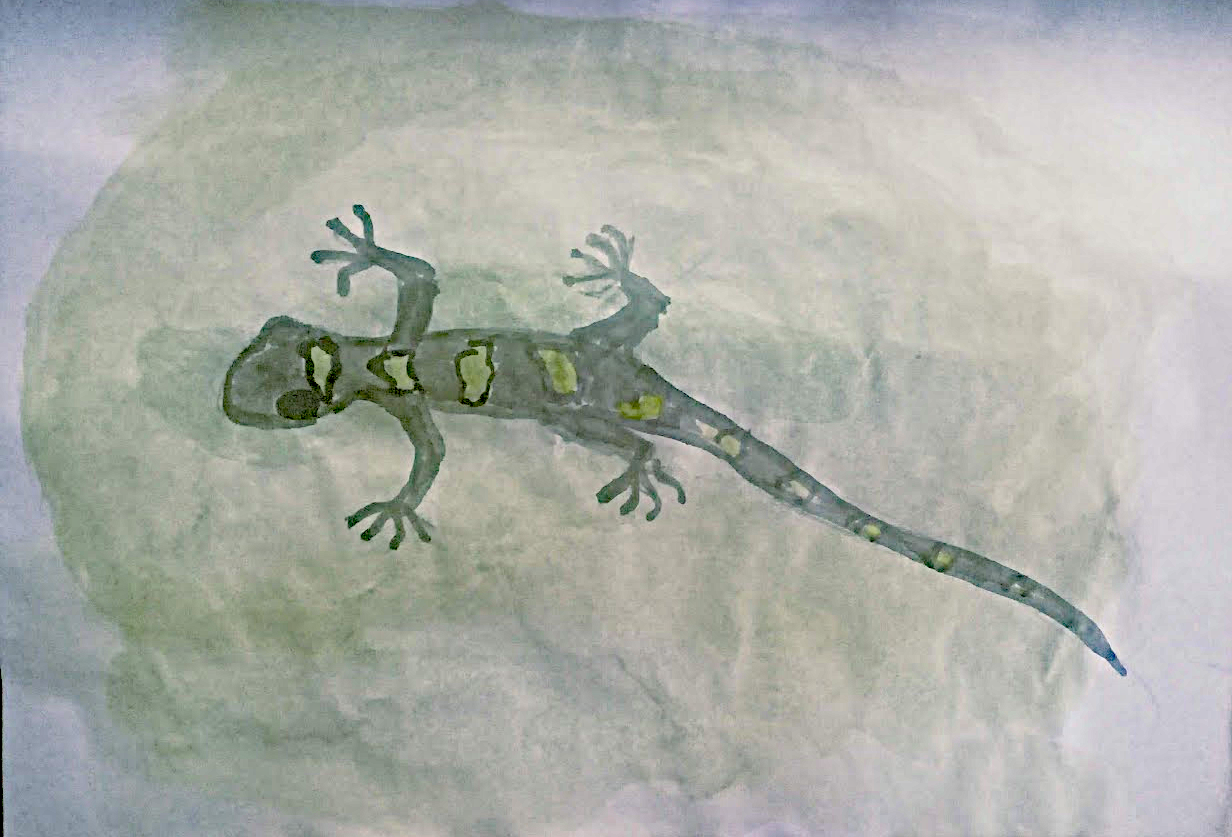
\includegraphics[height=.8\paperheight,angle=0]{lagartija}};
	
\end{tikzpicture}


\newpage
\begin{tikzpicture}[remember picture, overlay]
	\node [inner sep=0pt, minimum width=\paperwidth, minimum height=\paperheight,opacity=.8] at (current page.center) {
\includegraphics[width=\paperwidth,height=\paperheight,angle=0]{paper20}};
\end{tikzpicture}	

TAMBIÉN SE CONTRARIÓ CUANDO TIRÉ VARIAS MACETAS EN UNA DE MIS CORRIDAS, EN MI DEFENSA PUEDO DECIR QUE LA MACETA NO PARECÍA MUY SÓLIDA NI IMPORTANTE, CONTIENE UNOS YUYOS AMARGOS QUE COME CON AIRES DE GRAN GOURMET.

LE DICEN RÚCULA, SI SE LE PONE UN BUEN QUESO, PUEDE SER UNA BUENA COMBINACIÓN. EN OCASIONES ROBO ALGUNOS PEDAZOS DE PIZZA, Y LES CONFIESO QUE PUEDE SER UNA AGRADABLE COMBINACIÓN. 		¿VIERON LA PELÍCULA RATATOUILLE?



YO LA VI UN POCO, ME PARECE UN EXAGERADO HOMENAJE A LAS RATAS, PERO RESCATO QUE LA PELÍCULA DA GANAS DE PROBAR NUEVOS ALIMENTOS E INTENTAR COMBINAR COMIDAS CONOCIDAS. MIS CROQUETAS SABOR PESCADO PODRÍAN MEJORARSE SI PUSIÉRAMOS UN POCO DE ESFUERZO Y CREATIVIDAD.


\newpage
\begin{tikzpicture}[remember picture, overlay]
	\node [inner sep=0pt, minimum width=\paperwidth, minimum height=\paperheight,opacity=.8] at (current page.center) {
\includegraphics[width=\paperwidth,height=\paperheight,angle=0]{paper20}};
	
\end{tikzpicture}
PARA CONOCER UN TANTO MEJOR EL BARRIO, DECIDÍ REALIZAR UN MAPA QUE MOSTRARA LUGARES IMPORTANTES PARA MÍ. SÉ QUE LOS HUMANOS TIENEN MUCHAS PANTALLAS DONDE DESLIZAN SUS DEDOS Y HACE APARECER MAPAS, PERO YO CONFÍO EN LOS PAPELES. ESOS MISMOS PAPELES QUE ROMPO A VECES SIN MUCHA REFLEXIÓN, PUEDEN SERVIR PARA ESCRIBIR Y DIBUJAR. 

ASÍ ES, APROVECHANDO QUE MI PADRE INTENTA PINTAR CON TINTA CHINA --AÚN TIENE MUCHO QUE APRENDER-- HE REALIZADO ALGUNOS INTENTOS PARA DIBUJAR Y COLOREAR. PUES ¡GARRAS A LA OBRA!

\newpage
\begin{tikzpicture}[remember picture, overlay]
	\node [inner sep=0pt, minimum width=\paperwidth, minimum height=\paperheight,opacity=.8] at (current page.center) {
\includegraphics[width=\paperwidth,height=\paperheight,angle=0]{paper20}};
	\node [inner sep=0pt, minimum width=\paperwidth, minimum height=.5\paperheight,opacity=1,xshift=0\paperwidth,yshift=0\textheight] at (current page.center) {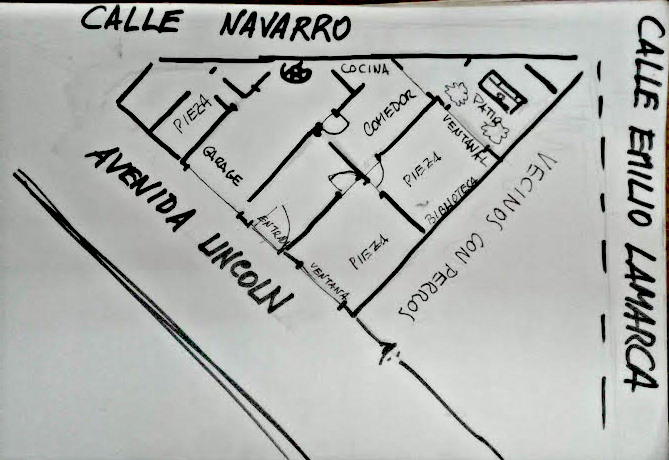
\includegraphics[height=.7\paperheight,angle=0]{plano_casa}};
	\node [inner sep=0pt, minimum width=.9\paperwidth, minimum height=\paperheight,opacity=1,xshift=0\paperwidth,text width=.95\linewidth,yshift=-.4\paperheight] at (current page.center) {PRIMERO UN PLANO APROXIMADO DE LA CASA.};
\end{tikzpicture}


\newpage
\begin{tikzpicture}[remember picture, overlay]
	\node [inner sep=0pt, minimum width=\paperwidth, minimum height=\paperheight,opacity=.8] at (current page.center) {
\includegraphics[width=\paperwidth,height=\paperheight,angle=0]{paper22}};
\end{tikzpicture}

DISFRUTO EN VERDAD DE CADA UNO DE LOS AMBIENTES. EL ANTIGUO GARAGE ES UNA SALA PARA ENTRAR QUE ES MUY GRANDE, CON UN CÓMODO SILLÓN E INCLUSO UN PIANO, DONDE ME RECUESTO CON GRAN TRANQUILIDAD. EN VERANO, SE ABREN LAS PEQUEÑAS VENTANAS DEL PORTÓN Y PUEDO INVESTIGAR LO QUE SUCEDE POR LA CALLE LINCOLN.

TAMBIÉN, ESTÁ LA PIEZA QUE TIENE UNA GRAN VENTANA QUE DA A LA ESQUINA DE LINCOLN Y NAVARRO, DESDE ALLÍ PUEDO SUBIRME AL BORDE Y OBSERVAR PERSONAS, ANIMALES, ÁRBOLES Y VEHÍCULOS.

LA COCINA JUNTO AL COMEDOR TAMBIÉN ES UN LUGAR IMPORTANTE, PUES POR EMPEZAR ESTÁ ALLÍ MI PLATO DE COMIDA Y MI PLATO DE AGUA.


\newpage
\begin{tikzpicture}[remember picture, overlay]
	\node [inner sep=0pt, minimum width=\paperwidth, minimum height=\paperheight,opacity=.8] at (current page.center) {
\includegraphics[width=\paperwidth,height=\paperheight,angle=0]{paper22}};
	\node [inner sep=0pt, minimum width=\paperwidth, minimum height=.5\paperheight,opacity=1,xshift=0.25\paperwidth,yshift=-.1\textheight] at (current page.center) {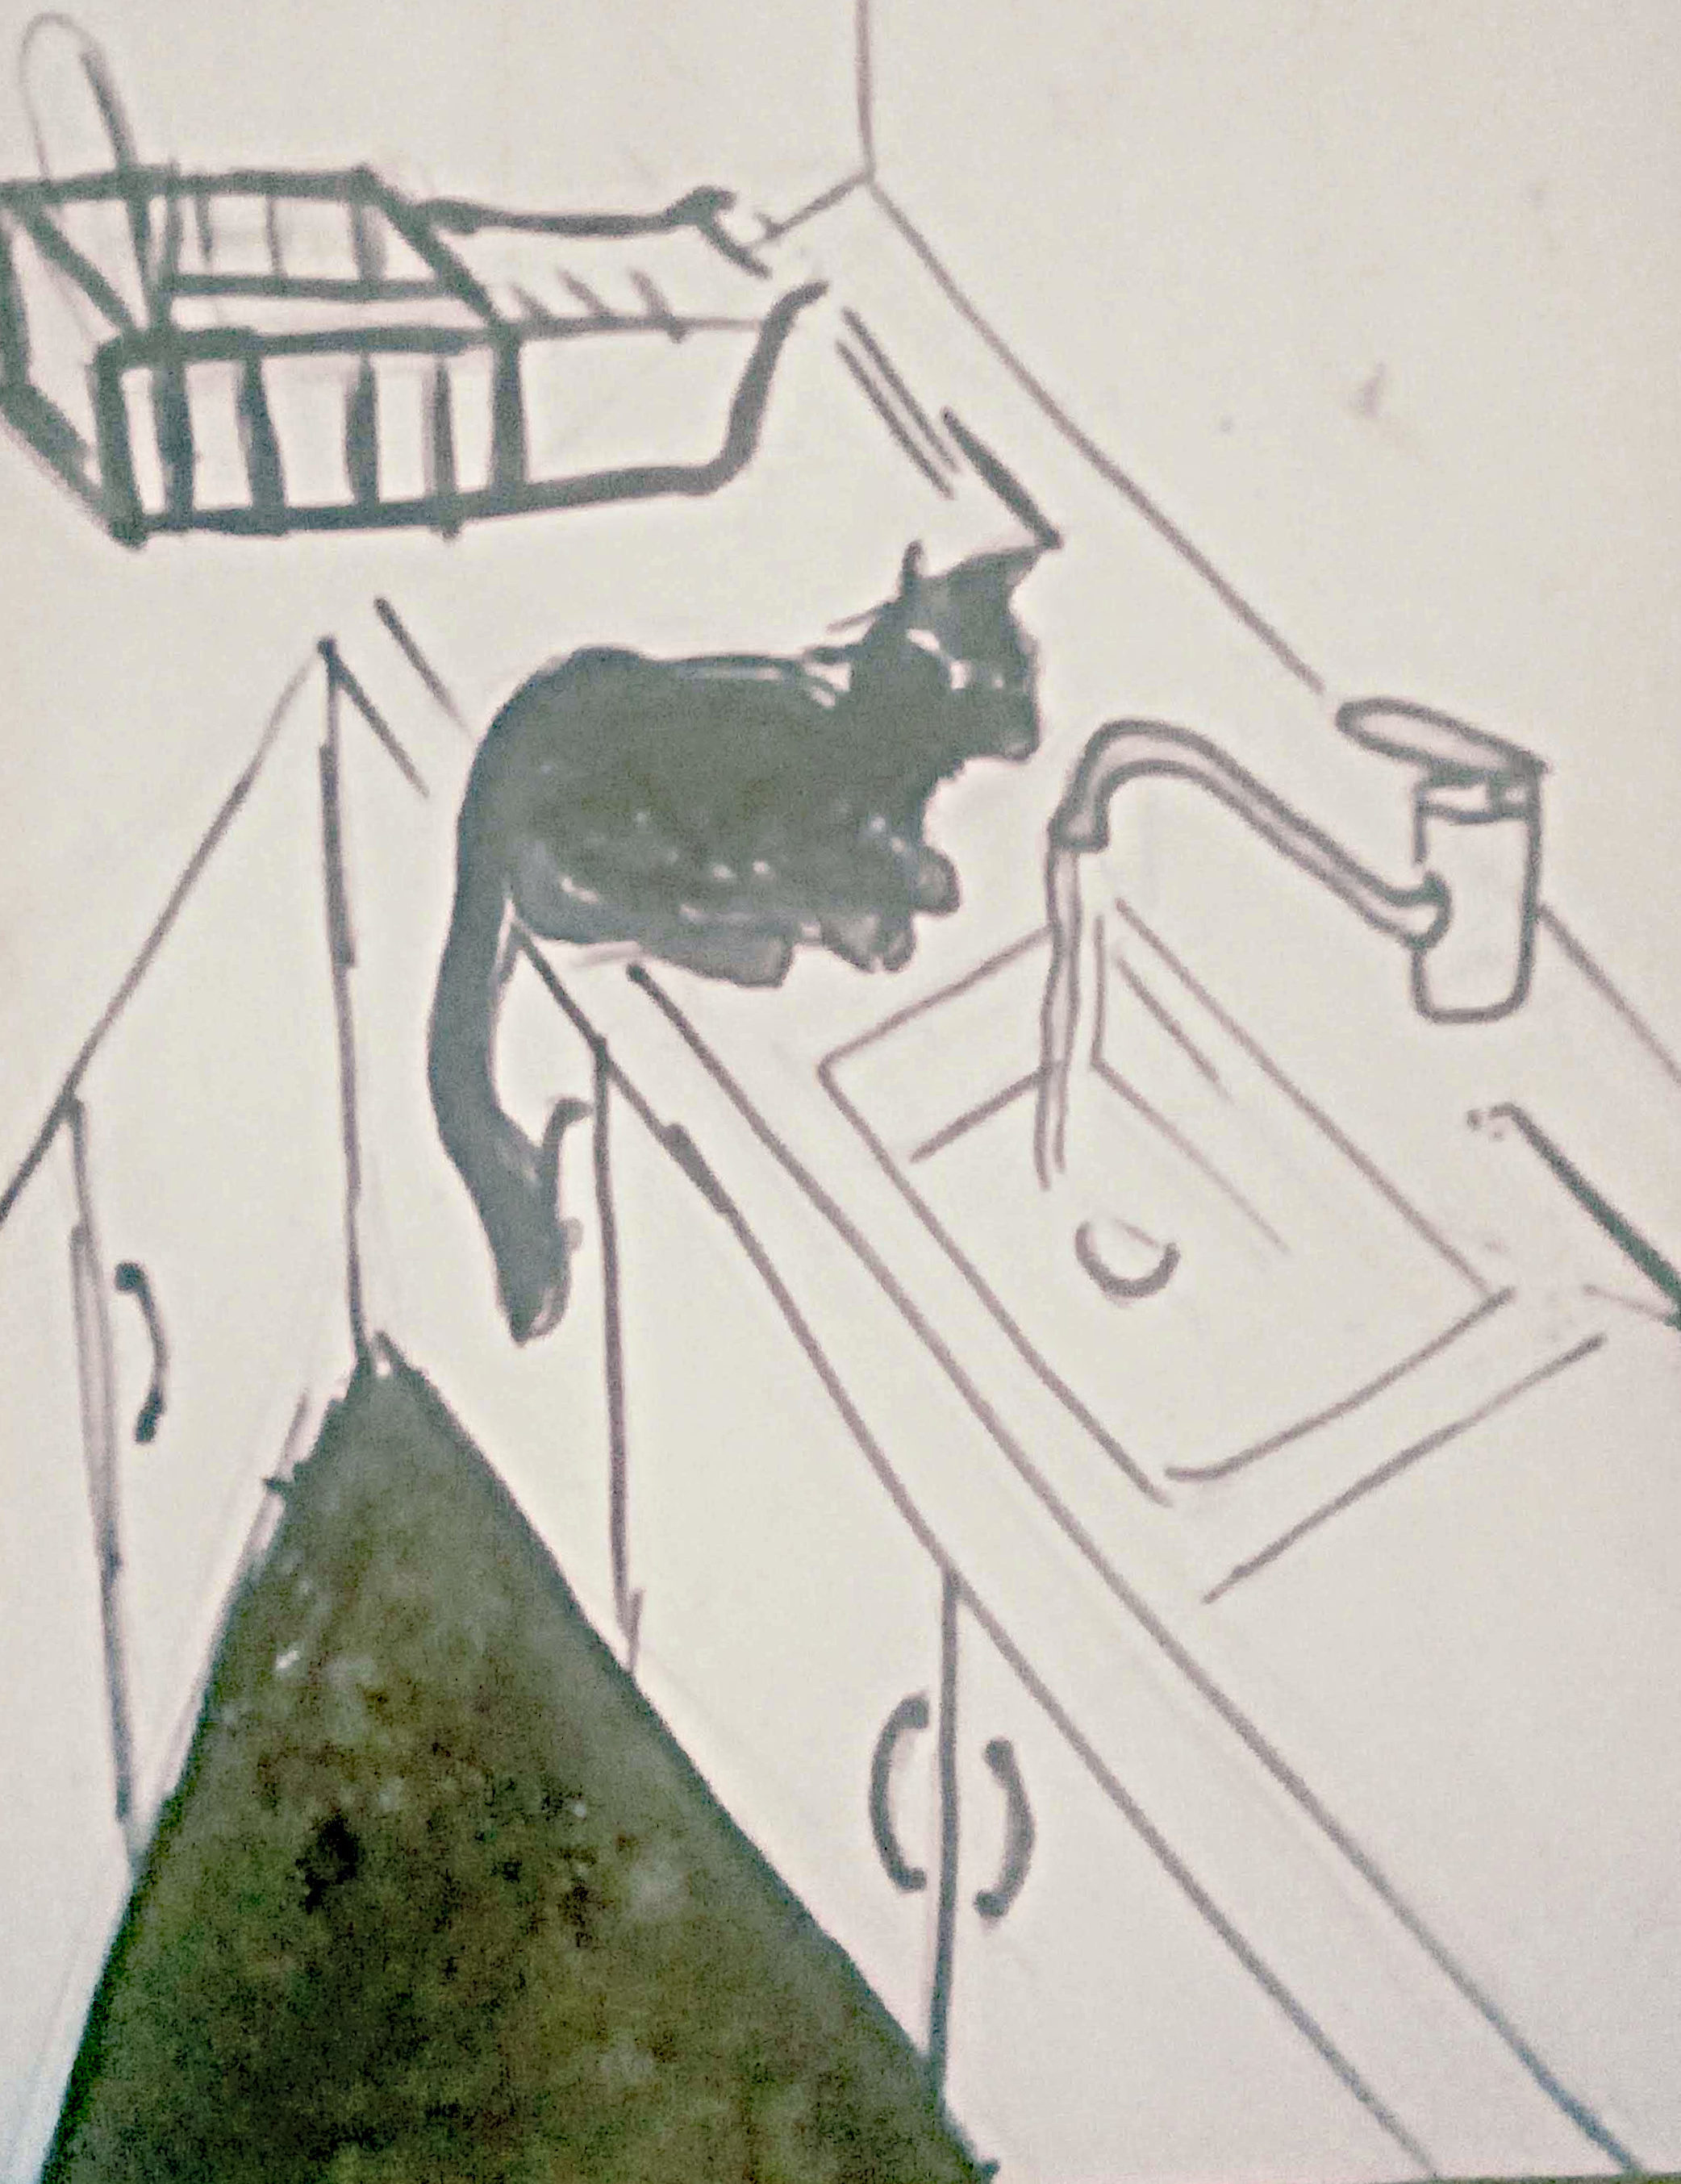
\includegraphics[height=.7\paperheight,angle=0]{cocina_agua}};	
	
	
	\node [inner sep=0pt, minimum width=.9\paperwidth, minimum height=\paperheight,opacity=1,xshift=-.03\paperwidth,text width=.9\linewidth,yshift=.35\paperheight] at (current page.center) {ME GUSTA SUBIRME A TODO LUGAR QUE SE PUEDA, Y POR ESO, PASEO POR MESAS Y MESADAS MIENTRAS ME LO PERMITEN. };
	\node [inner sep=0pt, minimum width=.9\paperwidth, minimum height=\paperheight,opacity=1,xshift=-.2\paperwidth,text width=.5\linewidth,yshift=-0.1\paperheight] at (current page.center) {	
		EN LA MESADA TENGO ACCESO AL AGUA QUE SALE DIRECTO DE LA CANILLA, ES UN IRRESISTIBLE PASATIEMPO CAZAR AL AGUA QUE NO DEJA DE DESCENDER Y SALPICAR. SI BIEN NO SOMOS MUY AMIGOS DE MOJARNOS, EN ESTA CONDICIÓN, UN GATO PUEDE ACEPTAR UNAS BUENAS GOTAS A CAMBIO DE MUCHOS MINUTOS DE DIVERSIÓN.  	
		
	};
\end{tikzpicture}
\newpage
\begin{tikzpicture}[remember picture, overlay]
	\node [inner sep=0pt, minimum width=\paperwidth, minimum height=\paperheight,opacity=.8] at (current page.center) {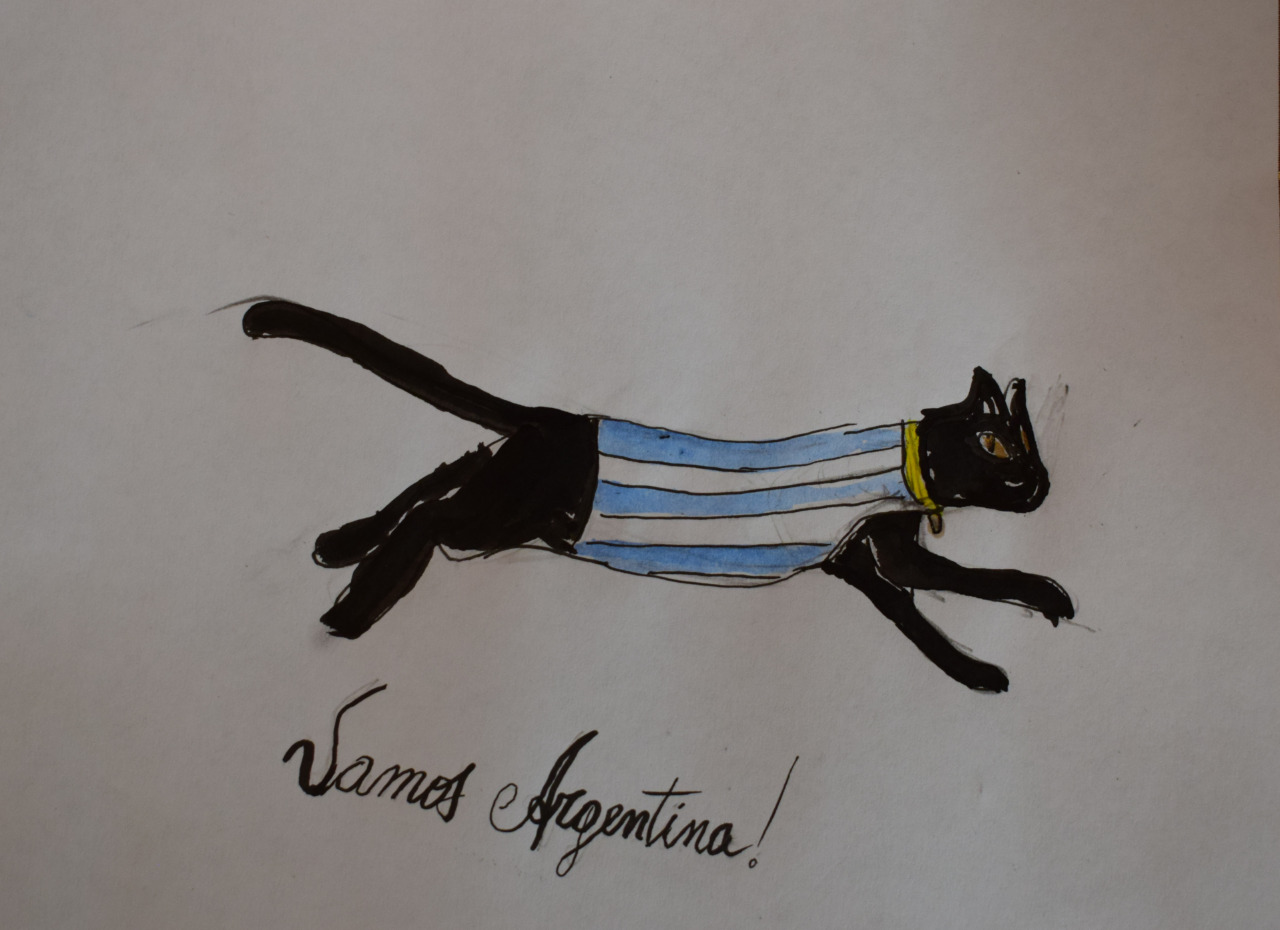
\includegraphics[width=\paperwidth,height=\paperheight,angle=0]{ottoko_arg}};
	
\end{tikzpicture}


\newpage
\begin{tikzpicture}[remember picture, overlay]
	\node [inner sep=0pt, minimum width=\paperwidth, minimum height=\paperheight,opacity=.8] at (current page.center) {
\includegraphics[width=\paperwidth,height=\paperheight,angle=0]{paper22}};
	\node [inner sep=0pt, minimum width=\paperwidth, minimum height=.5\paperheight,opacity=1,xshift=0\paperwidth,yshift=.1\textheight] at (current page.center) {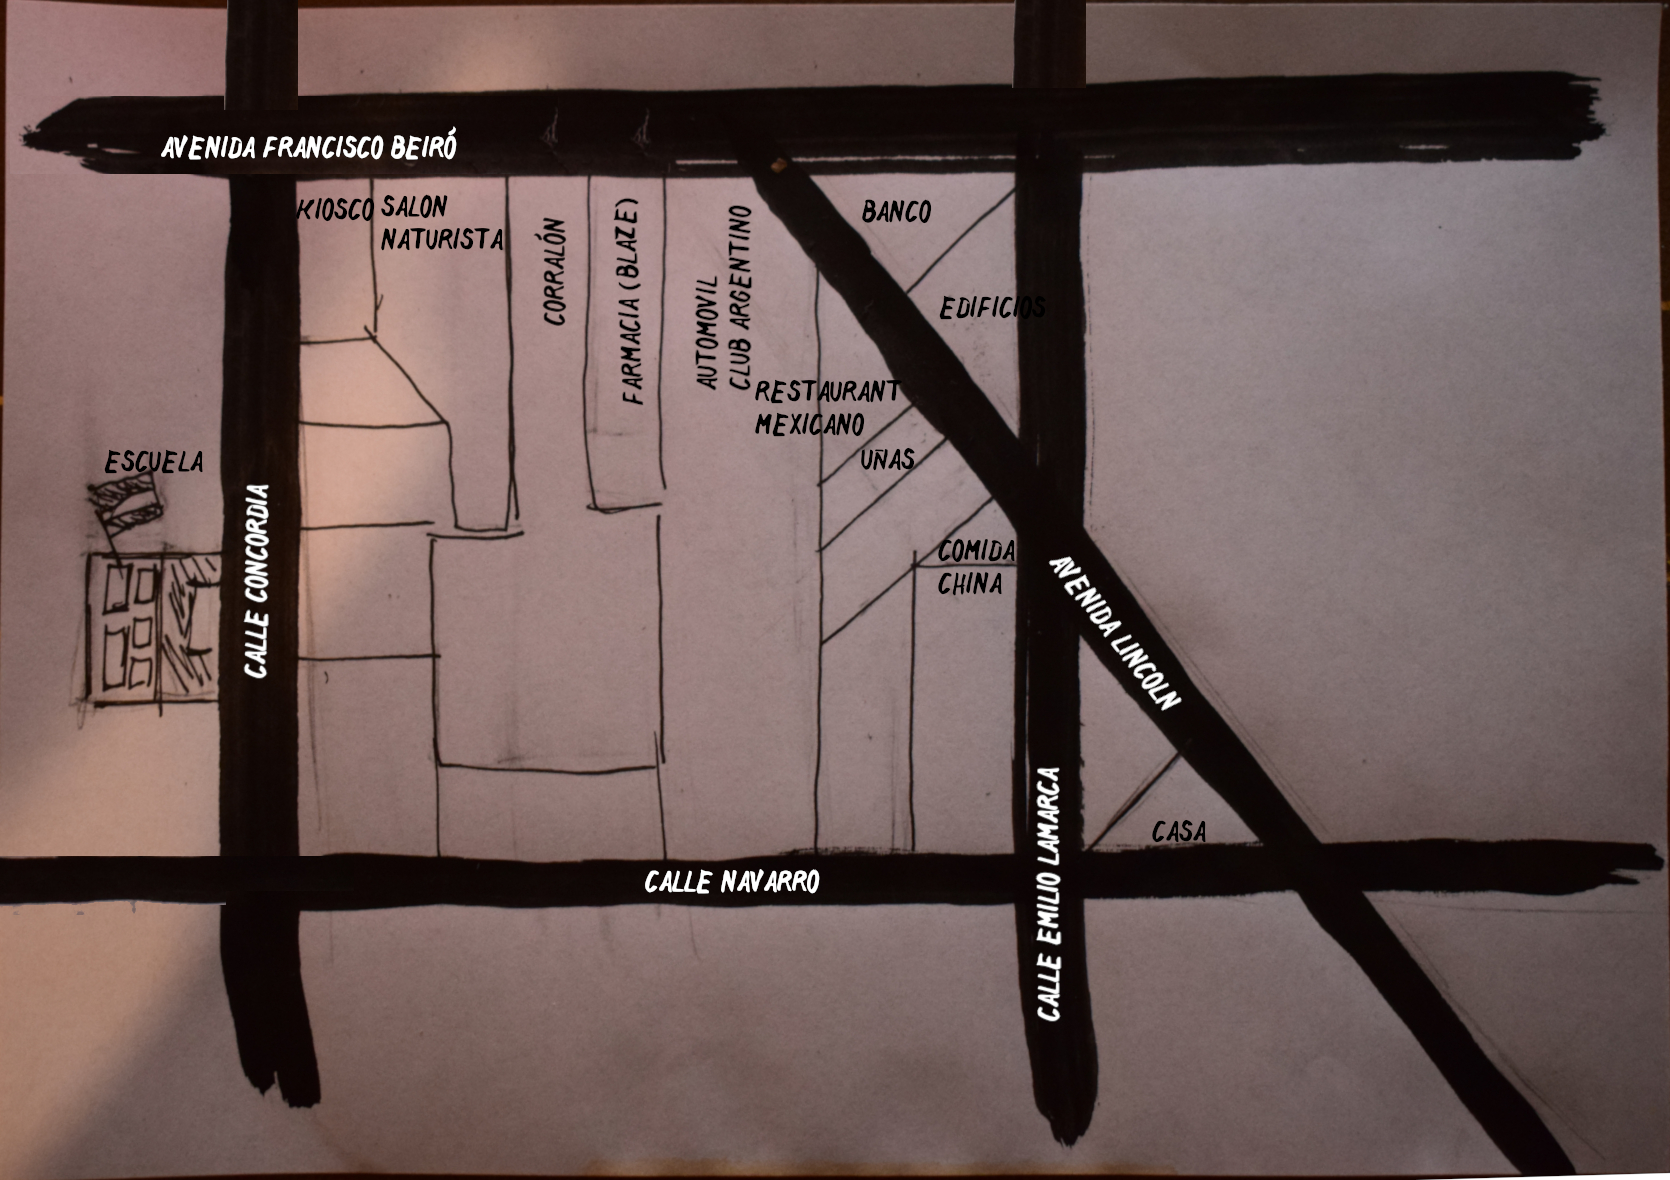
\includegraphics[height=.7\paperheight,angle=0]{plano2}};	
	
	\node [inner sep=0pt, minimum width=.9\paperwidth, minimum height=\paperheight,opacity=1,xshift=0\paperwidth,text width=.9\linewidth,yshift=-0.35\paperheight] at (current page.center) {	
		MÁS ALLÁ DE LA CASA, ESTÁ EL PLANO DE LAS CALLES QUE LA RODEAN. PUSE LOS LUGARES QUE FUI CONOCIENDO.};
\end{tikzpicture}


\newpage
\begin{tikzpicture}[remember picture, overlay]
	\node [inner sep=0pt, minimum width=\paperwidth, minimum height=\paperheight,opacity=1] at (current page.center) {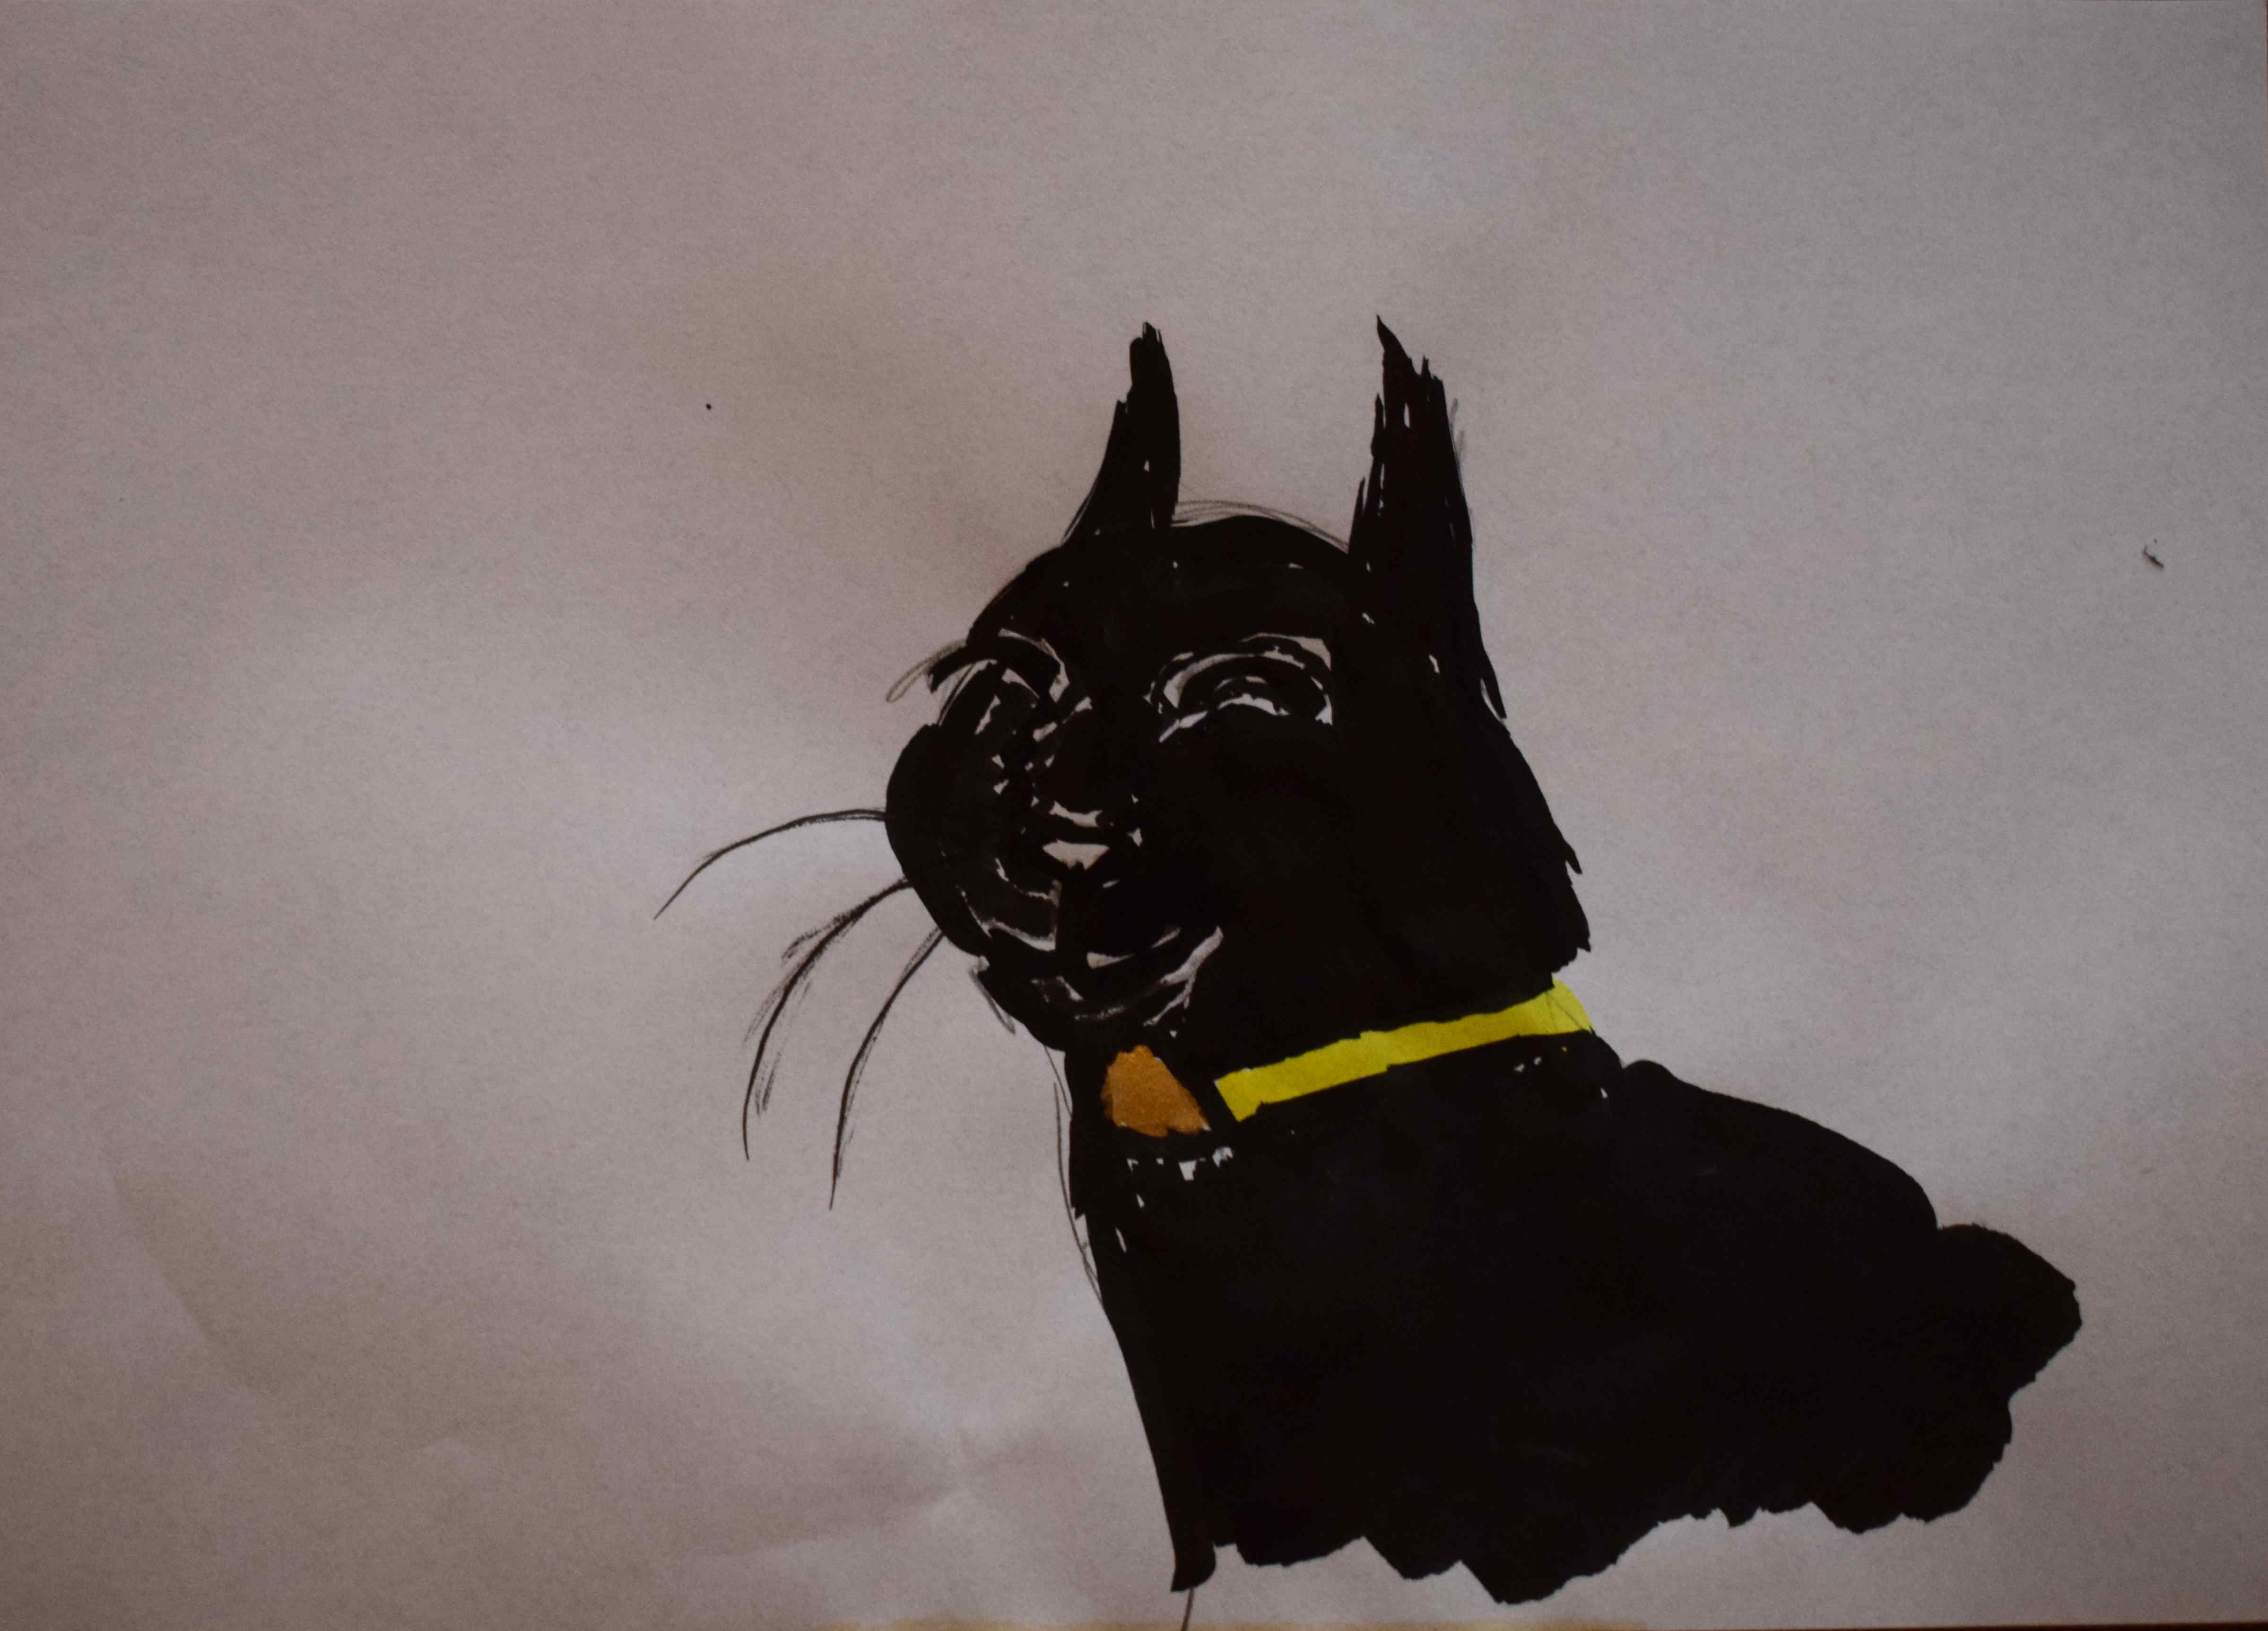
\includegraphics[width=\paperwidth,height=\paperheight,angle=0]{Ottoko_geometria}};
	
	
	\node [inner sep=0pt, minimum width=.9\paperwidth, minimum height=\paperheight,opacity=1,xshift=0\paperwidth,text width=.9\linewidth,yshift=0.\paperheight] at (current page.center) {	
		MIRANDO UN TANTO ESTOS PLANOS, ME FUI DANDO CUENTA DE LO IMPORTANTE QUE
		
		ES LA GEOMETRÍA.
		
		EN LAS FORMAS DE LAS 
		
		CASAS Y LAS CALLES
		
		ABUNDAN LOS 
		
		TRIÁNGULOS,
		
		LOS RECTÁNGULOS,
		
		LOS PARALELOGRAMOS,
		
		LOS TRAPECIOS, 
		
		TODO PUEDE LLEGAR A 
		
		PENSARSE COMO ALGO 
		
		DE DIBUJO SIMPLE.};
\end{tikzpicture}





\newpage
\begin{tikzpicture}[remember picture, overlay]
	\node [inner sep=0pt, minimum width=\paperwidth, minimum height=\paperheight,opacity=1] at (current page.center) {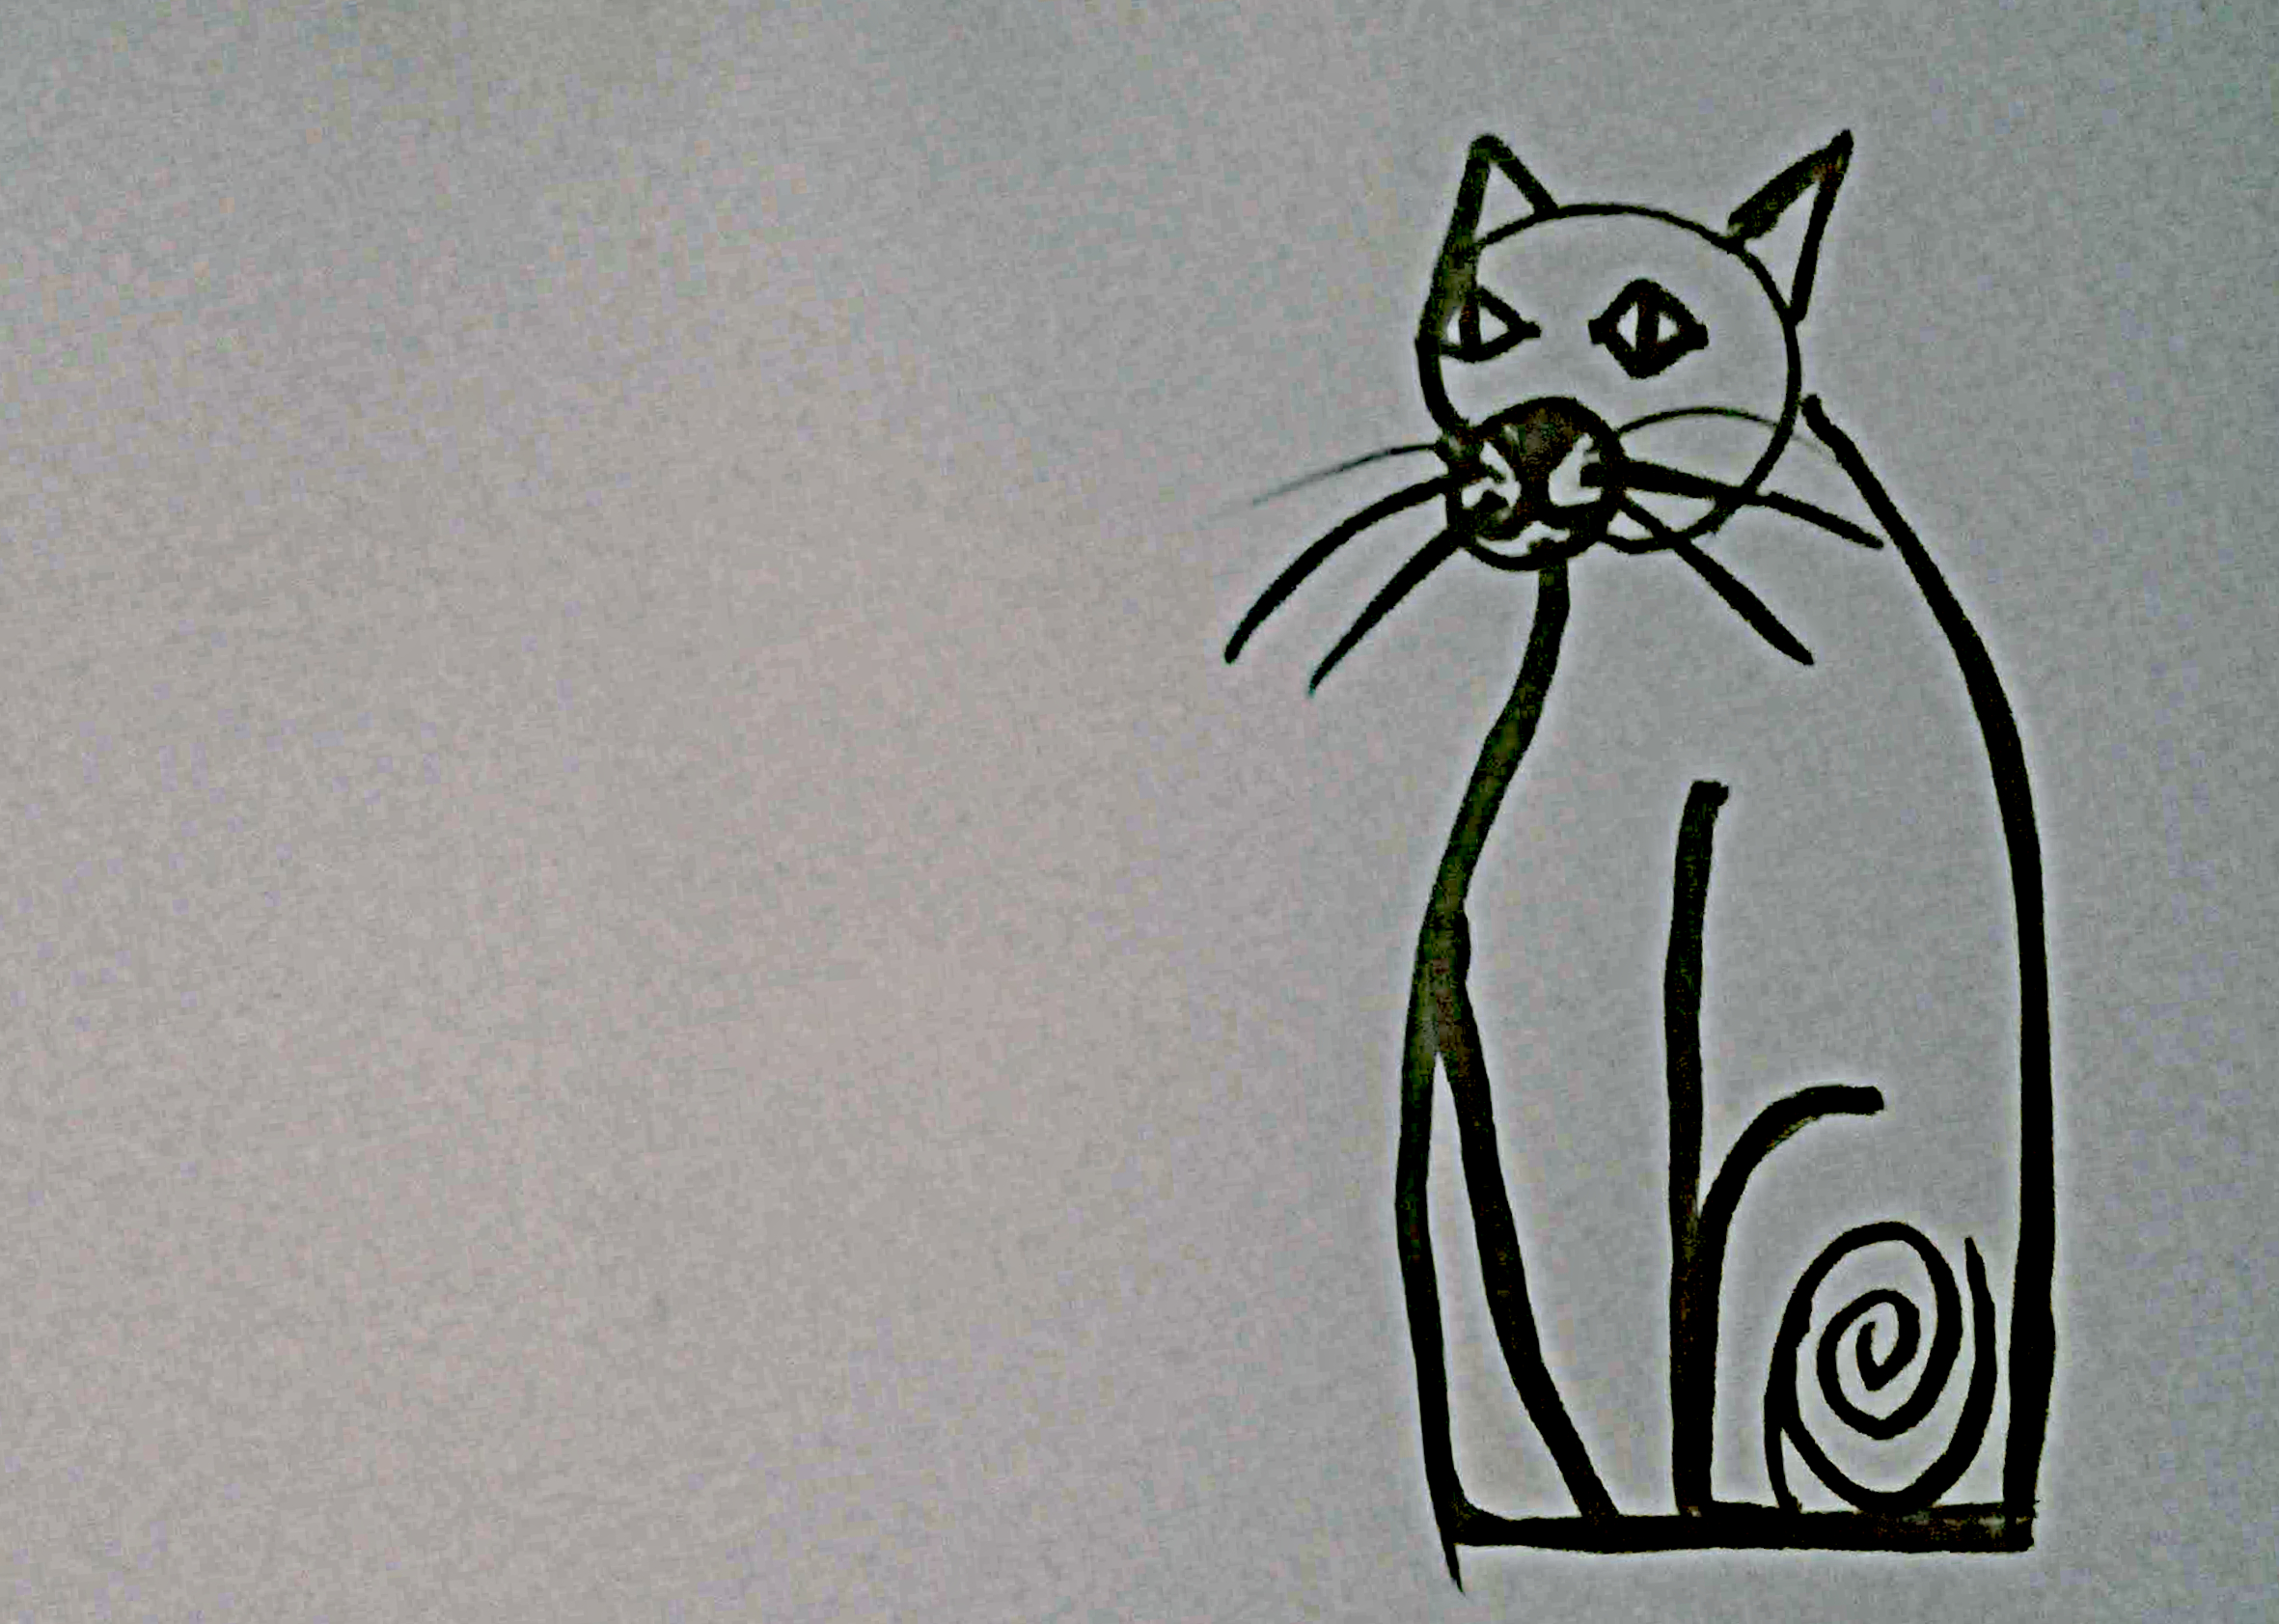
\includegraphics[width=\paperwidth,height=\paperheight,angle=0]{gato_geometrico}};
	
	
	\node [inner sep=0pt, minimum width=.9\paperwidth, minimum height=\paperheight,opacity=1,xshift=-.2\paperwidth,text width=.5\linewidth,yshift=0.\paperheight] at (current page.center) {	
		INCLUSO UN GATO!
		AQUÍ PINTÉ MUY SIMPLE 
		UNA ESPECIE DE GATO GEOMÉTRICO. CÍRCULOS, TRIÁNGULOS, ARCOS Y ESPIRAL.
		
		LAS ESPIRALES SON FIGURAS MUY INTERESANTES, COMO CIRCUNFERENCIAS QUE NUNCA TERMINAN DE CERRARSE. SI OBSERVAN BIEN, EN NUESTRA VIDA DE TODOS LOS DÍAS PODEMOS VER ESPIRALES.};
\end{tikzpicture}


\newpage
\begin{tikzpicture}[remember picture, overlay]
	\node [inner sep=0pt, minimum width=\paperwidth, minimum height=\paperheight,opacity=1] at (current page.center) {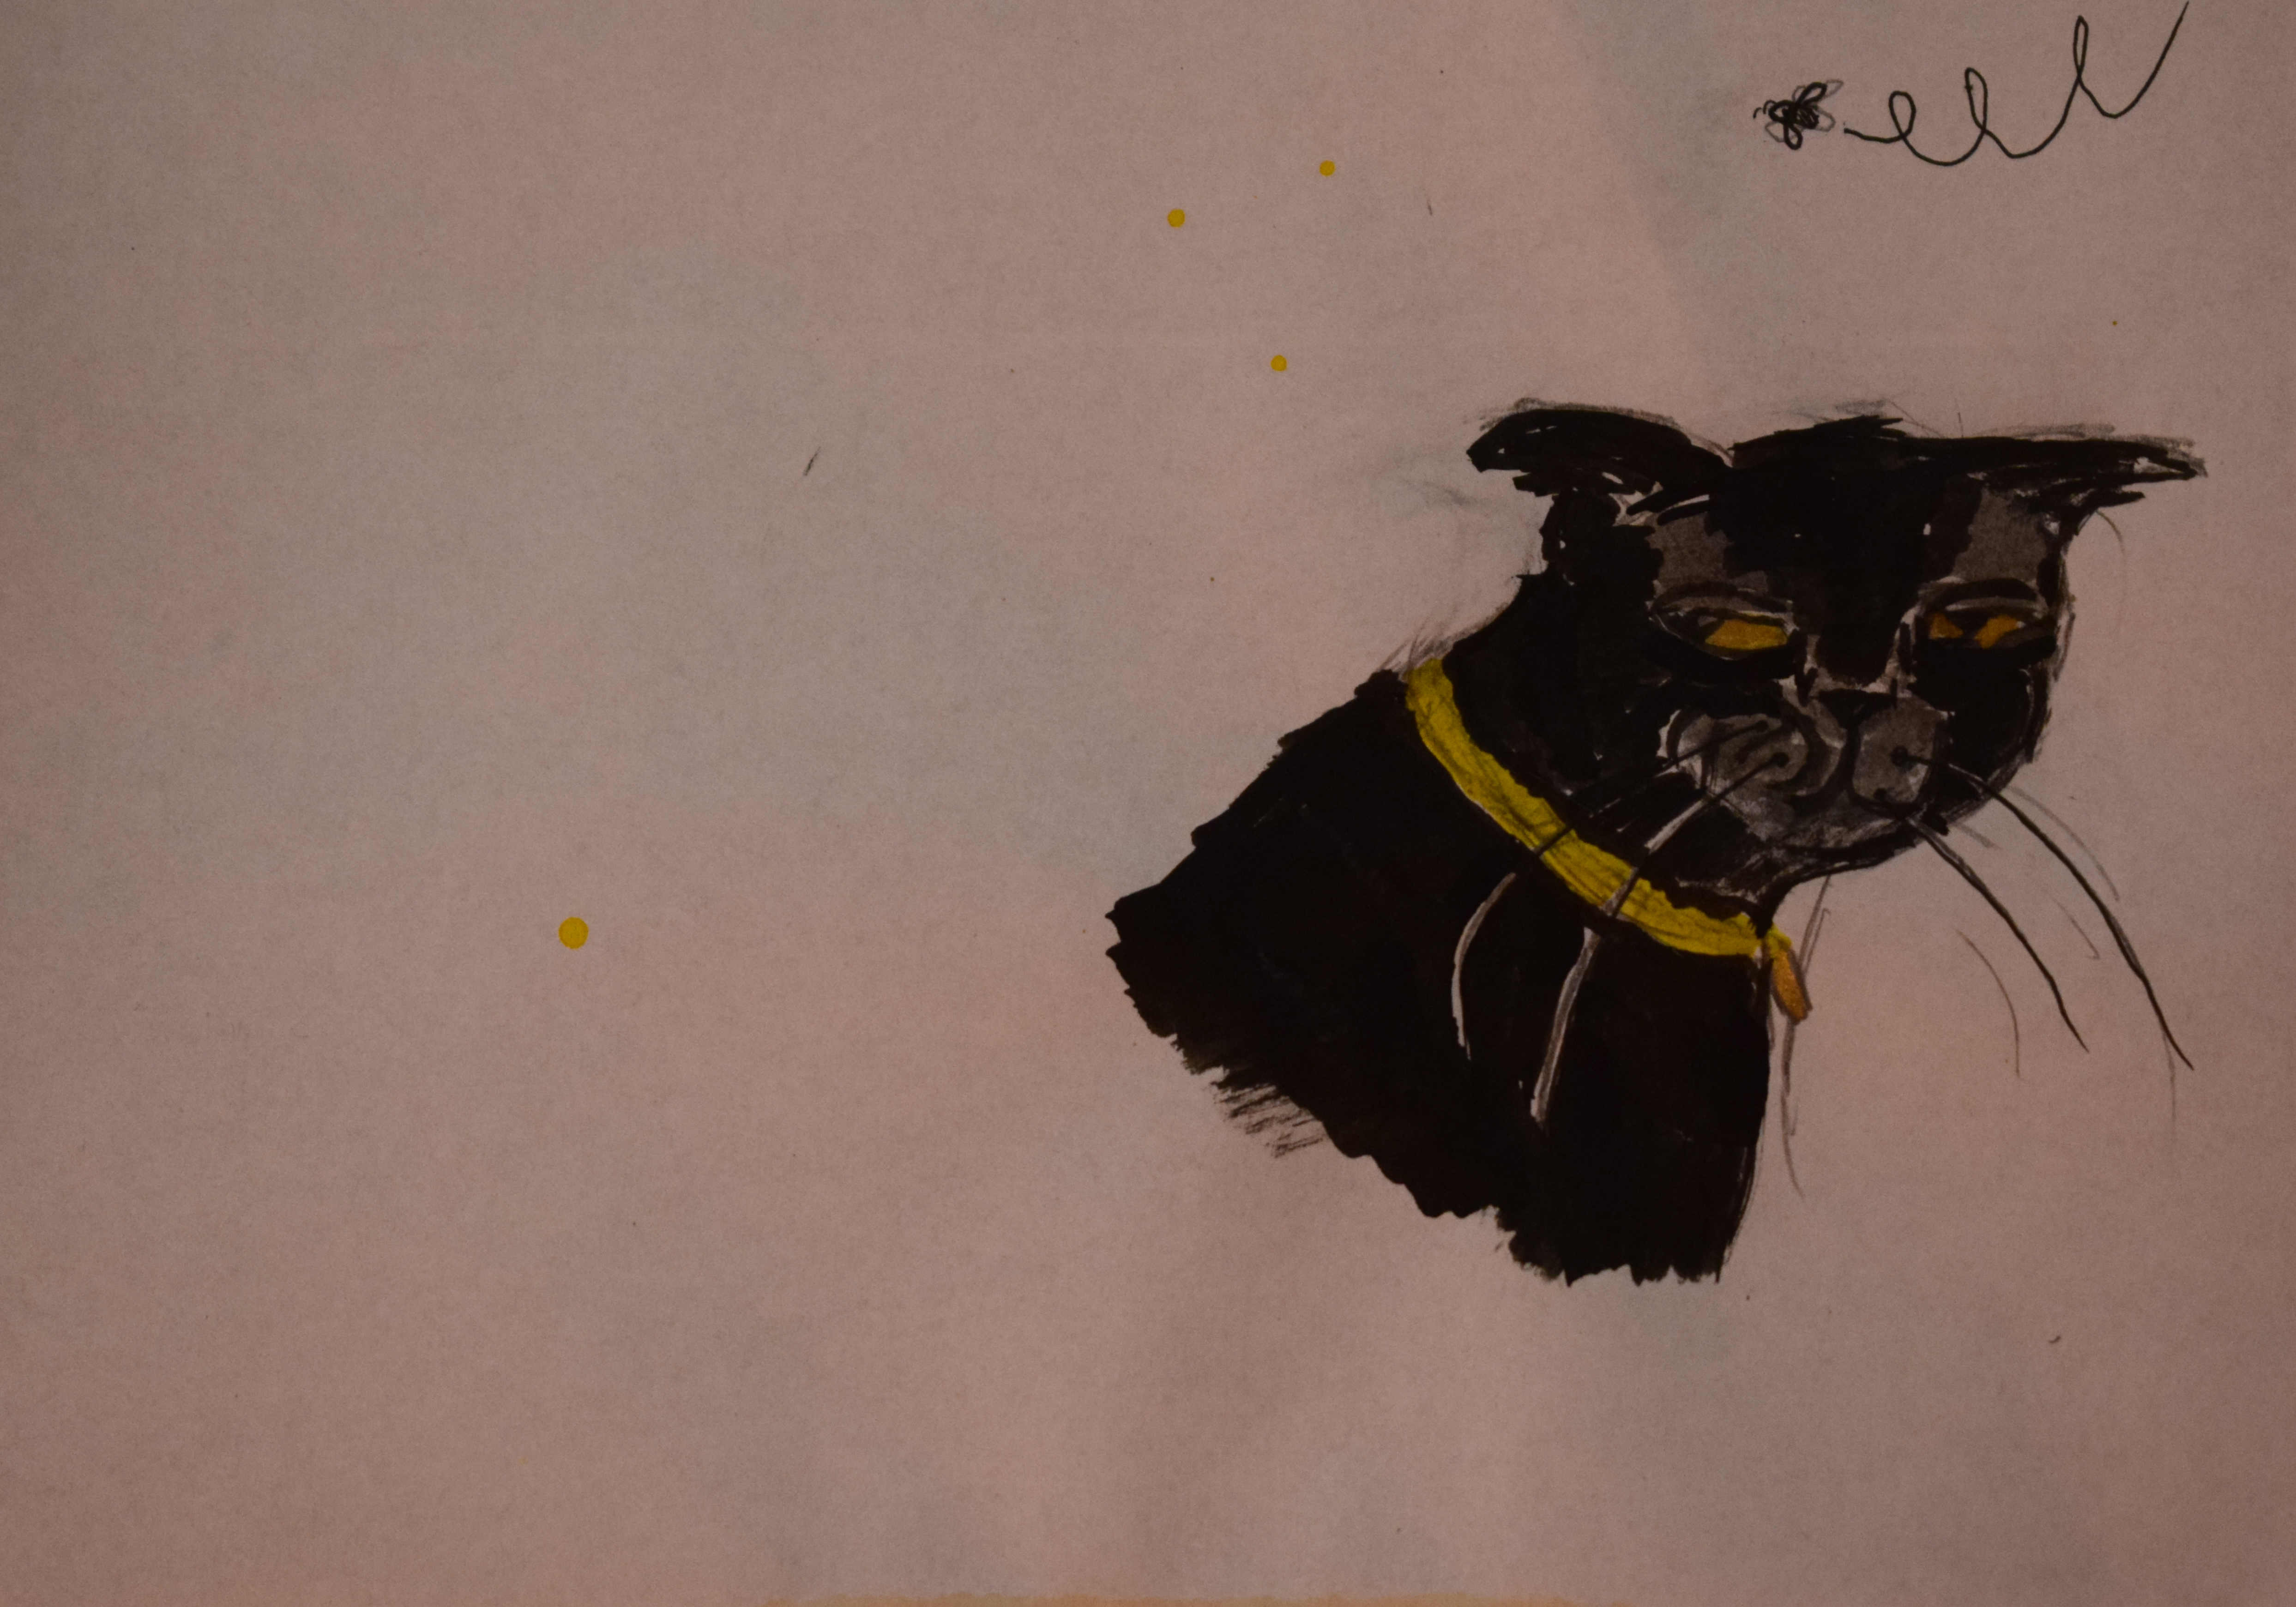
\includegraphics[width=\paperwidth,height=\paperheight,angle=0]{dormita}};
\end{tikzpicture}

VOY A CONTARLES ALGO QUE APRENDÍ UN DÍA DORMITANDO SOBRE LA BIBLIOTECA. 

ALGUNAS DE MIS MEJORES IDEAS LAS 

HE CONSEGUIDO HACIENDO SIESTAS ENTRE 

MIS LECTURAS. O LECTURAS ENTRE 

MIS SIESTAS.

¿NUNCA LES PASÓ DE QUEDARSE

DORMIDOS MIENTRAS ESTUDIAN?

PUES A MI MUCHO, Y UNA
DE LAS

IDEAS CURIOSAS QUE ENTENDÍ

FUE LA RELACIÓN ARMÓNICA 

QUE TIENEN LAS HOJAS DE PAPEL. Y QUE TIENE QUE VER CON ESPIRALES. 

\newpage
\begin{tikzpicture}[remember picture, overlay]
	\node [inner sep=0pt, minimum width=\paperwidth, minimum height=\paperheight,opacity=.6] at (current page.center) {
\includegraphics[width=\paperwidth,height=\paperheight,angle=0]{paper20}};
	
\end{tikzpicture}

LAS HOJAS QUE USAMOS PARA DIBUJAR O PARA IMPRIMIR EN NUESTRAS CASAS NO TIENEN UN TAMAÑO CUALQUIERA. SI SE FIJAN EN EL PAPEL QUE LAS ENVUELVE, DICE CLARAMENTE A4. SI NO TIENEN LA VISTA PRECISA DE UN FELINO, PUEDEN TOMAR UNA REGLA Y MEDIR SUS LADOS, VERÁN QUE SON DE 29,7 CM Y DE 21,0 CM.

SI DIVIDEN 29,7 $/$/ 21,0 $=$ 297 $/$ 210.

LES VA A DAR 1,414$\ldots$

EN REALIDAD, LAS MEDIDAS QUE DIJE ANTES NO SON LAS ABSOLUTAMENTE PRECISAS Y EL NÚMERO 1,414 ES UNO MUY ESPECIAL. LO PUEDEN ENCONTRAR SI DIBUJAN UN CUADRADO DE 1 CENTÍMETRO DE LADO. SI MIDEN LA DIAGONAL DEL CUADRADO, SE TRATA DE 1,414$\ldots$. PERO CLARO, ES MUY DIFÍCIL MEDIR BIEN ALGO TAN CHIQUITO... QUIZÁS CON UN MICROSCOPIO AL LADO O SACANDO UNA FOTO CON MUCHO ZOOM.


\newpage
\begin{tikzpicture}[remember picture, overlay]
	\node [inner sep=0pt, minimum width=\paperwidth, minimum height=\paperheight,opacity=.6] at (current page.center) {
\includegraphics[width=\paperwidth,height=\paperheight,angle=0]{paper20}};  	
	\node [inner sep=0pt, minimum width=.9\paperwidth, minimum height=\paperheight,opacity=1,xshift=.2\paperwidth,text width=.5\linewidth,yshift=0.\paperheight] at (current page.center) {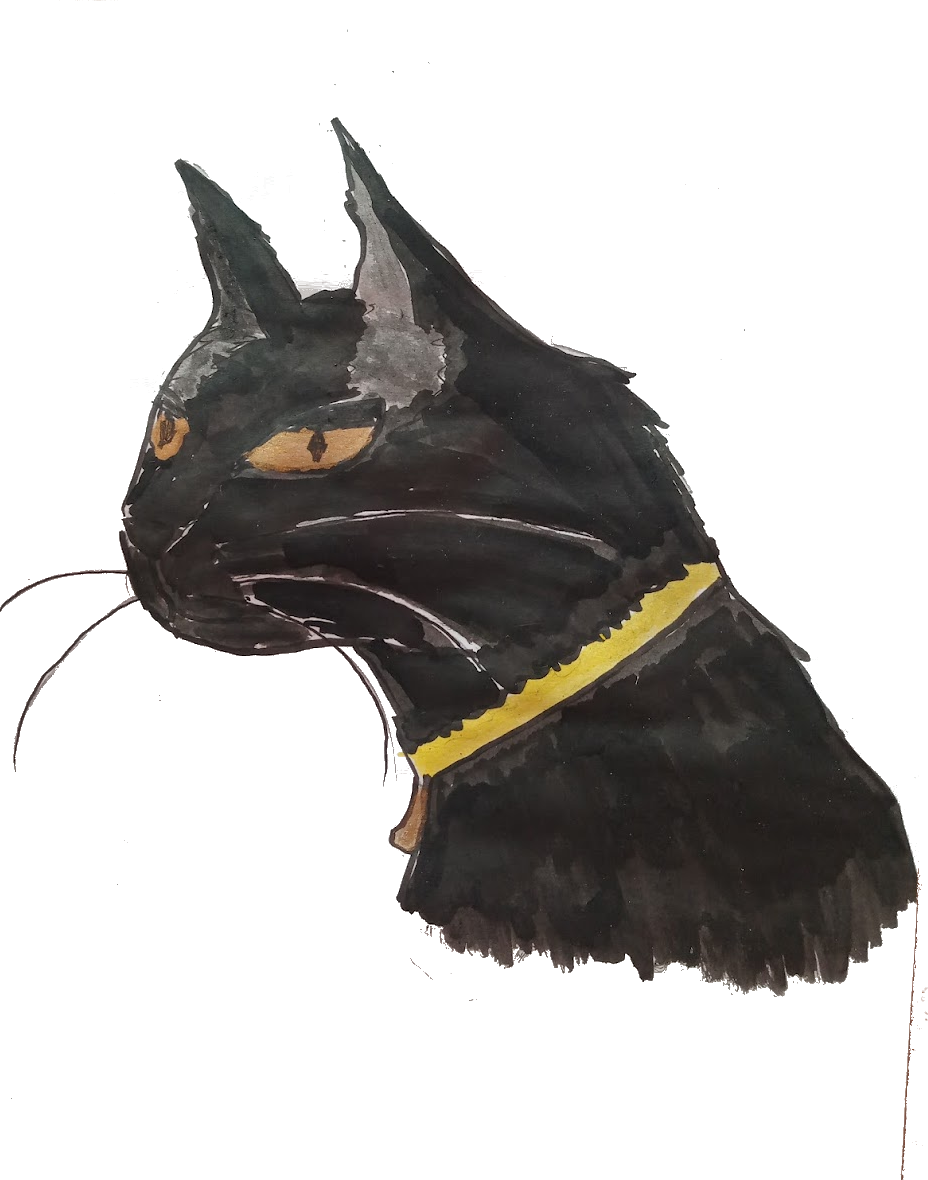
\includegraphics[width=.5\paperwidth,height=\paperheight,angle=0]{ottoko_piensa}};	
\end{tikzpicture}
LO QUE PODEMOS HACER, EN VEZ DE 

MEDIR LA DIAGONAL DE UN CUADRADO

DE 1 CENTÍMETRO DE LADO, ES MEDIR 

LA DIAGONAL DE UN CUADRADO DE 10

CENTÍMETROS DE LADO.

TENDRÁ QUE SER DE 14,1 CM.

PUES USTEDES, LOS HUMANOS,

SUELEN USAR REGLAS QUE 

ESTÁN A LO SUMO

EN MILÍMETROS, QUE SON LAS MÍNIMAS

DISTANCIAS QUE PUEDEN VER AL OJO.

PERO SEPAN QUE ENTRE DOS PUNTOS SIEMPRE 

PODEMOS ENCONTRAR OTRO PUNTO. AÚN MÁS ALLÁ 

DE LA PRECISIÓN FELINA.

\newpage

\begin{tikzpicture}[remember picture, overlay]
	\node [inner sep=0pt, minimum width=\paperwidth, minimum height=\paperheight,opacity=.6] at (current page.center) {
\includegraphics[width=\paperwidth,height=\paperheight,angle=0]{paper22}};
	
\end{tikzpicture}
EXISTEN LAS COSAS QUE PODEMOS VER CON NUESTROS PROPIOS OJOS Y AQUELLAS QUE PENSAMOS. UN PUNTO, SI LO DIBUJAMOS CON UN LÁPIZ O UN MARCADOR, SIEMPRE TENDRÁ UN ESPESOR O UNA TRAZA QUE TIENE QUE VER CON NUESTROS ÚTILES. ¿SABEN COMO PODRÍAN CREAR UN PUNTO MÁS ´´FINITO´´? 

CRUZANDO DOS PELOS.

ALLÍ DONDE SE CRUZAN PODRÍAMOS DECIR QUE EXISTE UN PUNTO. PERO HASTA LOS PELOS TIENEN UN ESPESOR CONSIDERABLE, ¡ALGO ASÍ COMO 1 MILÍMETRO DIVIDIDO 100!

ADEMÁS TAMBIÉN PODEMOS PENSAR EN FORMAS DE CUALQUIER TAMAÑO Y QUE NO PUEDE DIBUJARSE. POR EJEMPLO, CUADRADOS.

ES FÁCIL DIBUJAR UN CUADRADO DE 10 CM DE LADO, DE 1 CM DE LADO, PERO DE 1 MILÍMETRO? ¿O DE 0,01 MILÍMETRO?
\newpage
\begin{tikzpicture}[remember picture, overlay]
	\node [inner sep=0pt, minimum width=\paperwidth, minimum height=\paperheight,opacity=.6] at (current page.center) {
\includegraphics[width=\paperwidth,height=\paperheight,angle=0]{paper22}};	
	\node [inner sep=0pt, minimum width=.9\paperwidth, minimum height=\paperheight,opacity=1,xshift=0\paperwidth,text width=\linewidth,yshift=0.\paperheight] at (current page.center) {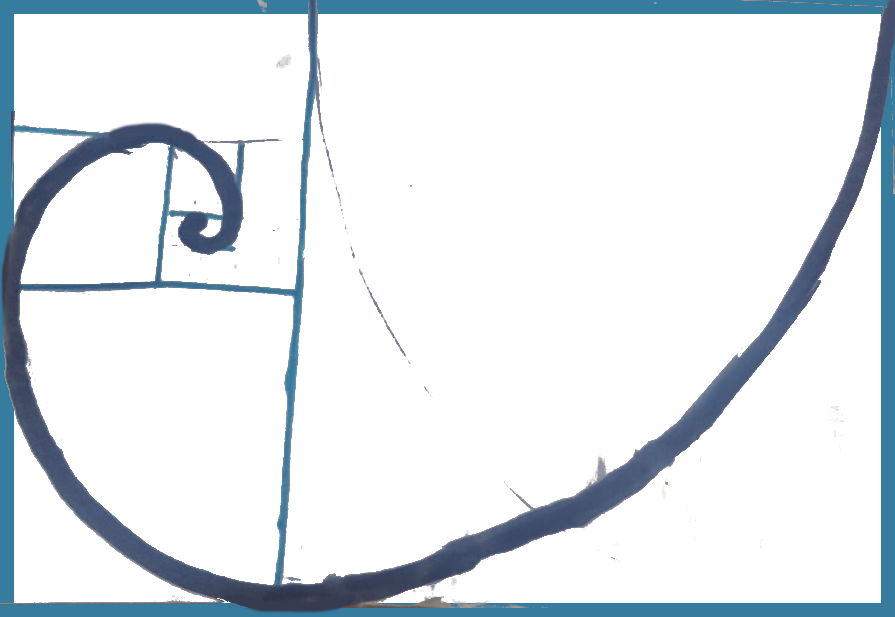
\includegraphics[width=.9\paperwidth,height=.9\paperheight,angle=0]{espiral1}}; 	
\end{tikzpicture}
\newpage
\begin{tikzpicture}[remember picture, overlay]
	\node [inner sep=0pt, minimum width=\paperwidth, minimum height=\paperheight,opacity=.6] at (current page.center) {
\includegraphics[width=\paperwidth,height=\paperheight,angle=0]{paper22}};
\end{tikzpicture}	
NO PODEMOS HACERLO CON NUESTROS ÚTILES HABITUALES, PERO ES POSIBLE. Y ASÍ, IMAGINARNOS MILES DE FORMAS QUE PUEDEN EXISTIR EN NUESTRO CEREBRO PERO NO SOBRE UNA HOJA DE PAPEL. 

SI MIRAN LA CURVA ESPIRAL QUE DIBUJÉ, PODRÁN ADIVINAR CASI COMO LA CONSTRUÍ. EMPECÉ CON UN RECTÁNGULO CON LADOS DE 10 CM Y 16 CM. CON LA MEDIDA DEL LADO MÁS CHICO, TRACÉ UN CUADRADO, DE 10 CM. ME QUEDA UN RECTÁNGULO MÁS PEQUEÑO AHORA DE 10 CM Y 6 CM. DE NUEVO DIBUJO UN CUADRADO AHORA DE 6 CM DE LADO, Y ME QUEDA UN RECTANGULITO DE 4 CM POR 6 CM. Y PODRÍA CONTINUAR HASTA QUE NO PUEDA DIBUJAR MÁS CUADRADITOS.

SI SE FIJAN, EN CADA CUADRADO HAY UN ARCO DE CIRCUNFERENCIA, Y ESE ARCO CAMBIA SU RADIO CUANDO CAMBIO DE CUADRADO, ASÍ TERMINÉ DIBUJANDO UNA ESPIRAL.

PERO NO ES CUALQUIER TIPO DE ESPIRAL.
\newpage
\begin{tikzpicture}[remember picture, overlay]
	\node [inner sep=0pt, minimum width=\paperwidth, minimum height=\paperheight,opacity=.6] at (current page.center) {
\includegraphics[width=\paperwidth,height=\paperheight,angle=0]{paper22}};
	\node [inner sep=0pt, minimum width=.9\paperwidth, minimum height=\paperheight,opacity=1,xshift=.25\paperwidth,text width=.5\linewidth,yshift=0.\paperheight] at (current page.center) {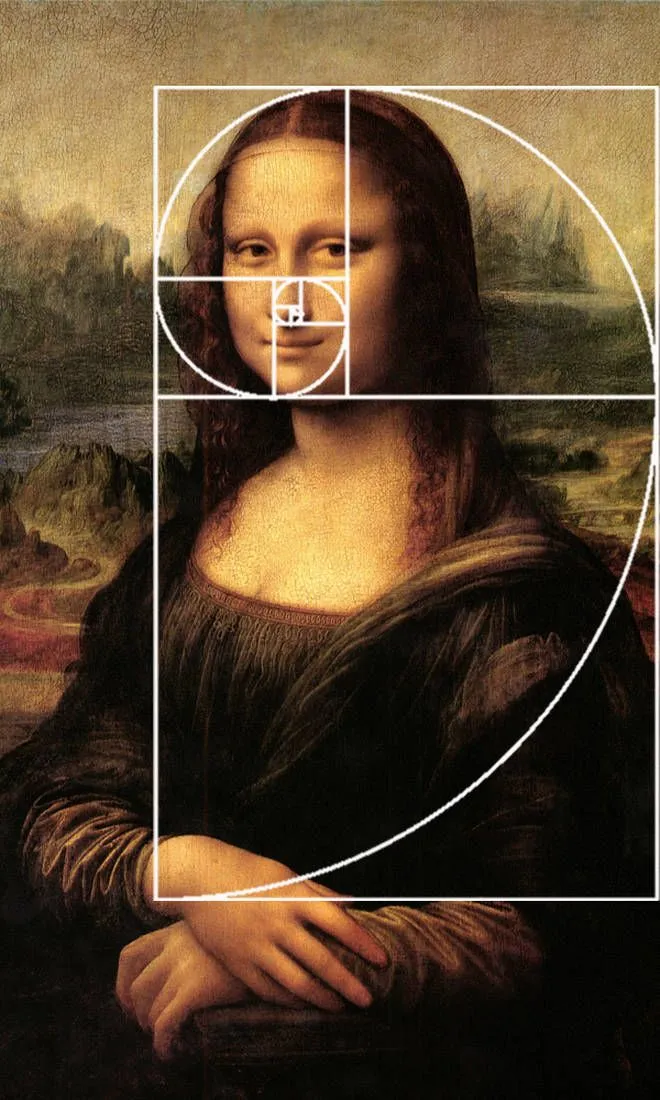
\includegraphics[width=.4\paperwidth,angle=0]{gioconda}};	
\end{tikzpicture}
ES LA ESPIRAL DE LA PROPORCIÓN

ÁUREA O DE ´´ORO´´.

¿´´ORO´´, DIJE? ¿PODRÉ HACER ORO

CON ESA FIGURA?

NO$\ldots$, Y ¡SI!

MIREN EL MAGNÍFICO CUADRO,

LA GIOCONDA DE LEONARDO

DA VINCI.

ALGUIEN LE DIBUJÓ UNA 

ESPIRAL DE ORO ENCIMA.

SÓLO PARA PROBAR QUE EL

GRAN ARTISTA, USÓ ESA 

PROPORCIÓN PARA QUE NOS

PAREZCA ARMÓNICA Y BELLA.

\newpage
\begin{tikzpicture}[remember picture, overlay]
	\node [inner sep=0pt, minimum width=\paperwidth, minimum height=\paperheight,opacity=.6] at (current page.center) {
\includegraphics[width=\paperwidth,height=\paperheight,angle=0]{paper23}};
\end{tikzpicture}
PODRÁN ENTENDER Y CREAR FORMAS BELLAS CONOCIENDO ESTE PEQUEÑO SECRETO QUE TIENE ALGO DE MATEMÁTICO. UN GATO CON TIEMPO LIBRE Y MUCHOS LIBROS A SU ALCANCE PUEDE PENSAR EN ESTAS COSAS Y COMPARTIRLAS CON QUIENES AMA. AÚN CUANDO PAREZCAN OCULTA, HAY MUCHA BELLEZA A NUESTRO ALREDEDOR Y ESO HACE A NUESTRA VIDA MÁS AGRADABLE, COMO CUANDO NOS DETENEMOS A OLER UNA FLOR, A ESCUCHAR LA CORRIENTE DE UN RÍO O LAS OLAS DEL MAR. EL VIENTO QUE SILVA ENTRE LOS ÁRBOLES Y NUESTRAS CONSTRUCCIONES.

PEQUEÑAS Y GRANDES ESCALAS DEL ESPACIO Y DEL TIEMPO. SABEN JUSTO HOY FESTEJAMOS QUE LA TIERRA ACABA DE DAR UNA VUELTA COMPLETA ALREDEDOR DEL SOL. ¡ES AÑO NUEVO! 
\newpage
\begin{tikzpicture}[remember picture, overlay]
	\node [inner sep=0pt, minimum width=\paperwidth, minimum height=\paperheight,opacity=.3] at (current page.center) {
\includegraphics[width=\paperwidth,height=\paperheight,angle=0]{paper23}};
	\node [inner sep=0pt, minimum width=.9\paperwidth, minimum height=\paperheight,opacity=1,xshift=.25\paperwidth,text width=.5\linewidth,yshift=0.\paperheight] at (current page.center) {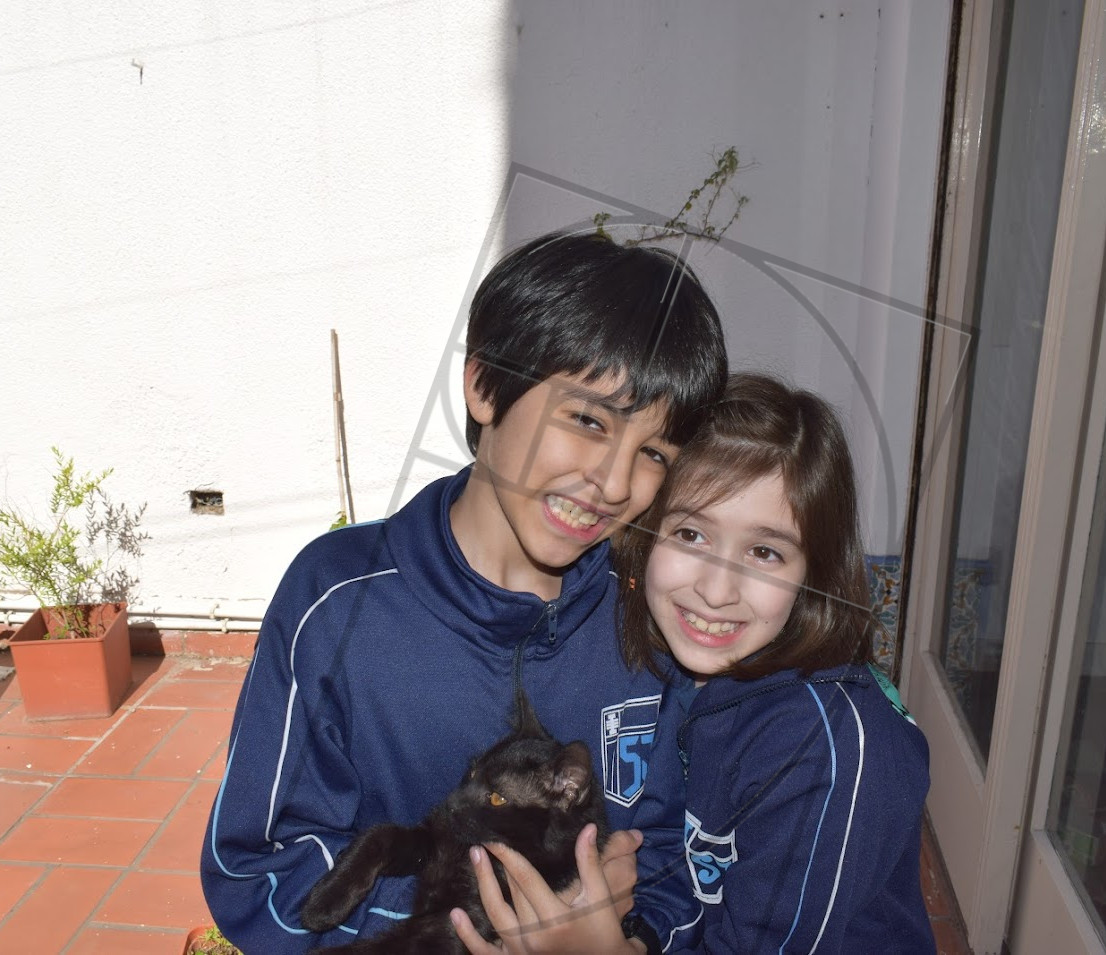
\includegraphics[width=.4\paperwidth,angle=0]{alegria_patio}};	
	\node [inner sep=0pt, minimum width=.9\paperwidth, minimum height=\paperheight,opacity=1,xshift=0\paperwidth,text width=.5\linewidth,yshift=-.35\paperheight] at (current page.center) { {\large¡OTTOKO Y PAPÁ LES DESEAN MUY FELIZ AÑO!}};	 	
\end{tikzpicture}

\vspace{.2\textheight}
\begin{minipage}{.5\textwidth}
	Y AUNQUE PAREZCA LEJOS Y HACE MUCHO, SEPAN QUE HAY BELLEZA, VERDAD Y AMOR AÚN DONDE NO SE IMAGINAN. QUE ESPERA PACIENTE SER DESCUBIERTO POR USTEDES CUANDO LA OPORTUNIDAD SE PRESENTE.
	
\end{minipage}

\newpage
\begin{tikzpicture}[remember picture, overlay]
	\node [inner sep=0pt, minimum width=\paperwidth, minimum height=\paperheight,opacity=.3] at (current page.center) {
\includegraphics[width=\paperwidth,height=\paperheight,angle=0]{paper23}};
	\node [inner sep=0pt, minimum width=.9\paperwidth, minimum height=\paperheight,opacity=1,xshift=-.25\paperwidth,text width=.5\linewidth,yshift=0.\paperheight] at (current page.center) {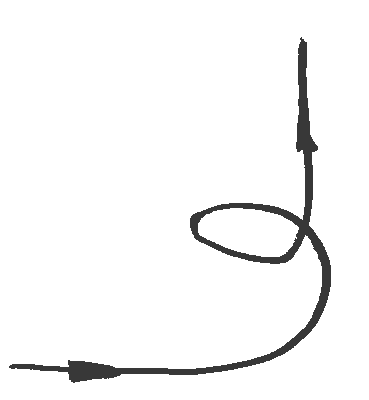
\includegraphics[width=.3\paperwidth,angle=0]{espiral2}};
	\node [inner sep=0pt, minimum width=.9\paperwidth, minimum height=\paperheight,opacity=1,xshift=.25\paperwidth,text width=.5\linewidth,yshift=0.\paperheight] at (current page.center) {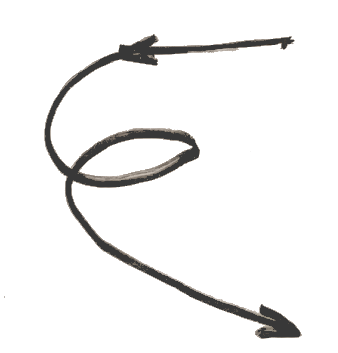
\includegraphics[width=.3\paperwidth,angle=0]{espiral3}};	
\end{tikzpicture}
PENSANDO EN ESPIRALES, SEGURO LAS RECONOCERÁN EN EL DISEÑO DE ESCALERAS. PERMITEN UNIR DIRECCIONES EN LAS 3 DIMENSIONES.
\vspace{.5\paperheight}

EN MI CASA HAY UNA BELLA ESCALERA DE TIPO ESPIRAL. ME GUSTA ESCAPAR PARA IR A VISITAR A LAS PERRITAS LUNA Y CHUBI, PERO SUELEN ATRAPARME ANTES DE QUE PUEDA SALUDARLAS.
